\Problem{Crate, Brick, Box, and Car FBDs}{\CrateBrickBoxCar}{
	For the following exercises, draw the situation and identify and name all the forces acting on the object. Then, using the particle model, draw a free-body diagram for the object. Include the direction of the net force $ \vec{F}_{net} $. Neglect air resistance.
}
\ProblemSub{\Crate}{
	(a) A heavy crate is being lowered straight down at a constant speed by a steel cable.
}
\Solution{\CrateFig}{
	\begin{figure}[h]
		\centering
		\begin{tikzpicture}
			\begin{scope}[shift={(-2,0)}]
				%\draw[thick] (-1,1) -- (1,1) -- (1,-1) -- (-1,-1) -- cycle;
				\filldraw[gray] (-0.8,0.8) -- (0.8,0.8) -- (0.8,-0.8) -- (-0.8,-0.8) -- cycle;
				\filldraw[lightgray] (-1,1) -- (-0.45,1) -- (-0.45,0.7) arc (90:180:0.25) -- (-1,0.45) -- cycle;
				\filldraw[lightgray,rotate=90] (-1,1) -- (-0.45,1) -- (-0.45,0.7) arc (90:180:0.25) -- (-1,0.45) -- cycle;
				\filldraw[lightgray,rotate=180] (-1,1) -- (-0.45,1) -- (-0.45,0.7) arc (90:180:0.25) -- (-1,0.45) -- cycle;
				\filldraw[lightgray,rotate=270] (-1,1) -- (-0.45,1) -- (-0.45,0.7) arc (90:180:0.25) -- (-1,0.45) -- cycle;
				\draw[red] (-0.8,0) -- (0.8,0);
				\draw[red] (0,-0.8) -- (0,0.8);
				\filldraw[lightgray] (-0.9,0.25) -- (-0.7,0.25) -- (-0.7,-0.25) -- (-0.9,-0.25) -- cycle;
				\filldraw[lightgray,rotate=90] (-0.9,0.25) -- (-0.7,0.25) -- (-0.7,-0.25) -- (-0.9,-0.25) -- cycle;
				\filldraw[lightgray,rotate=180] (-0.9,0.25) -- (-0.7,0.25) -- (-0.7,-0.25) -- (-0.9,-0.25) -- cycle;
				\filldraw[lightgray,rotate=270] (-0.9,0.25) -- (-0.7,0.25) -- (-0.7,-0.25) -- (-0.9,-0.25) -- cycle;
				\filldraw[lightgray] (0,0) circle (0.4);
				\filldraw[red] (-0.2,0.05) arc (180:0:0.1) arc (180:0:0.1) -- (0,-0.15) -- cycle;
				\draw[ultra thick] (0,0.9) -- (0,2);
				\node[anchor=north] at (0,-1) {gravity, $\vec{F}^{g}_{cr,E}$};
				\node[anchor=west] at (0,1.5) {tension, $\vec{F}^{T}_{cr,cb}$};
			\end{scope}
			\FBDaxes{2,0}{0}{axes}
			\FBDvectorXY{axes}{0,1}{FT}
			\node[anchor=west] at (FTtip) {$\vec{F}^{T}_{cr,cb}$};
			\FBDvectorXY{axes}{0,-1}{FG}
			\node[anchor=west] at (FGtip) {$\vec{F}^{g}_{cr,E}$};
			\FBDdot{axes}
			\node at ($(axes) + (1.5,0.5)$) {$\vec{F}^{net}=\vec{0}$};
		\end{tikzpicture}
	\end{figure}
}
\ProblemSub{\Brick}{
	(b) A brick is falling from the roof a three-story building.
}
\Solution{\BrickFig}{
	\begin{figure}[h]
		\centering
		\begin{tikzpicture}
			\begin{scope}[shift={(-3,0)}]
				\filldraw[gray,draw=black,thick] (-1,-2) -- (1,-2) -- (1,1) -- (-1,1) -- cycle;
				\draw[thick] (-0.3,-2) -- (0.3,-2) -- (0.3,-1.3) -- (-0.3,-1.3) -- cycle;
				\draw[thick,shift={(0.5,1)}] (-0.3,-2) -- (0.3,-2) -- (0.3,-1.3) -- (-0.3,-1.3) -- cycle;
				\draw[thick,shift={(-0.5,1)}] (-0.3,-2) -- (0.3,-2) -- (0.3,-1.3) -- (-0.3,-1.3) -- cycle;
				\draw[thick,shift={(0.5,2)}] (-0.3,-2) -- (0.3,-2) -- (0.3,-1.3) -- (-0.3,-1.3) -- cycle;
				\draw[thick,shift={(-0.5,2)}] (-0.3,-2) -- (0.3,-2) -- (0.3,-1.3) -- (-0.3,-1.3) -- cycle;
			\end{scope}
			\filldraw[red,draw=black,thick,shift={(-1,0)}] (-0.2,-0.1) -- (0.2,-0.1) -- (0.2,0.1) -- (-0.2,0.1) -- cycle;
			\draw (-1.2,0.15) -- (-1.2,0.3);
			\draw (-0.8,0.15) -- (-0.8,0.3);
			\draw (-1.1,0.15) -- (-1.1,0.4);
			\draw (-0.9,0.15) -- (-0.9,0.4);
			\node[anchor=north] at (-0.8,-0.1) {gravity, $\vec{F}^{g}_{br,E}$};
			\FBDaxes{2,0}{0}{axes}
			\FBDvectorXY{axes}{0,-1}{FG}
			\node[anchor=west] at (FGtip) {$\vec{F}^{g}_{br,E}$};
			\FBDdot{axes}
			\FBDvectorXY{$(axes)+(1.5,1.5)$}{0,-1}{Fnet}
			\node[anchor=west] at ($(Fnettip) + (0,0.5)$) {$\vec{F}^{net}$};
		\end{tikzpicture}
	\end{figure}
}
\ProblemSub[34]{\PushBox}{
	(c) A girl is pushing a box across a rough horizontal floor at a steadily increasing speed.
}
\Solution{\PushBoxFig}{We will use the subscript $S$ (as in ``surface'') for the floor.
	
	\begin{figure}[h]
		\centering
		\begin{tikzpicture}
			\node at (-3.5,0) {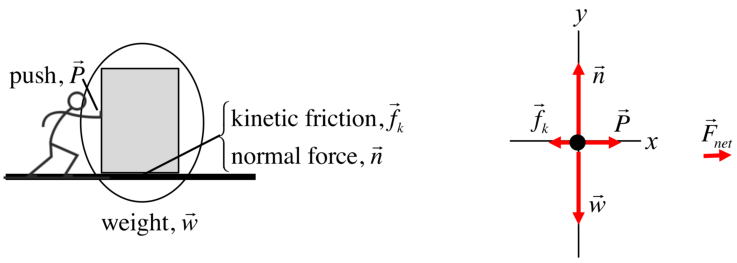
\includegraphics[trim={0 0 5cm 0},clip]{\FileDepth/Activities/Crate_Brick_Box_Car_FBDs/Girl_Pushing_the_Box_with_FBD}};
			\filldraw[white,shift={(-7.1,0.7)}] (0,0) rectangle (1.3,0.5);
			\node[anchor=south east] at (-5.7,0.7) {normal force, $\vec{F}^{N}_{BG}$};
			\filldraw[white,shift={(-5.6,-1.8)}] (0,0) rectangle (1.7,0.5);
			\node[anchor=south west] at (-5.6,-1.8) {gravity, $\vec{F}^{g}_{BE}$};
			\filldraw[white,shift={(-1,-0.6)}] (0,0) rectangle (0.5,0.5);
			\node[anchor=west] at (-1,-0.45) {$\vec{F}^{N}_{BS}$};
			\filldraw[white,shift={(-0.7,0)}] (0,0) rectangle (0.5,0.5);
			\node[anchor=west] at (-0.7,0.2) {$\vec{F}^{kf}_{BS}$};
			\FBDaxes{2.3,0}{0}{axes}
			\FBDvectorXY{axes}{0,-1.5}{FG}
			\node[anchor=west] at (FGtip) {$\vec{F}^{g}_{BE}$};
			\FBDvectorXY{axes}{0,1.5}{FNg}
			\node[anchor=west] at (FNgtip) {$\vec{F}^{N}_{BS}$};
			\FBDvectorXY{axes}{1,0}{FNp}
			\node[anchor=north] at (FNptip) {$\vec{F}^{N}_{BG}$};
			\FBDvectorXY{axes}{-0.5,0}{FK}
			\node[anchor=north] at (FKtip) {$\vec{F}^{kf}_{BS}$};
			\FBDvectorXY{$(axes)+(1.5,1)$}{0.5,0}{Fnet}
			\node[anchor=south] at (Fnettip) {$\vec{F}^{net}$};
			\FBDdot{axes}
		\end{tikzpicture}
	\end{figure}
}
\ProblemSub{\Brakes}{
	(d) You've slammed on your car brakes while going down a hill. The car is skidding to a stop.
}
\Solution{\BrakesFig}{
	\begin{figure}[h]
		\centering
		\begin{tikzpicture}
			\node at (-2.3,0) {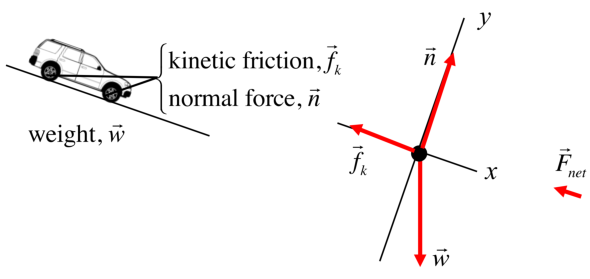
\includegraphics[trim={0 0 4.51cm 0},clip]{\FileDepth/Activities/Crate_Brick_Box_Car_FBDs/Car_Skidding_Downhill_with_FBD}};
			\filldraw[white,shift={(0.1,0.5)}] (0,0) rectangle (0.5,0.5);
			\node[anchor=west] at (0.4,1.3) {$\vec{F}^{kf}_{BS}$};
			\node[anchor=west] at (0.1,0.7) {$\vec{F}^{N}_{BS}$};
			\filldraw[white,shift={(-4.6,-0.2)}] (0,0) rectangle (1.7,0.5);
			\node[anchor=south west] at (-4.6,-0.2) {gravity, $\vec{F}^{g}_{BE}$};
			\FBDaxes{3,0}{-30}{axes}
			\FBDvectorMA{axes}{1.2}{150}{FK}
			\node[anchor=south] at (FKtip) {$\vec{F}^{kf}_{CS}$};
			\FBDvectorMA{axes}{1.5}{60}{FN}
			\node[anchor=west] at (FNtip) {$\vec{F}^{N}_{CS}$};
			\FBDvectorXY{axes}{0,-1.7}{FG}
			\node[anchor=north] at (FGtip) {$\vec{F}^{g}_{CE}$};
			\FBDvectorMA{$(axes)+(2,0)$}{0.4}{150}{Fnet}
			\node[anchor=south] at (Fnettip) {$\vec{F}^{net}$};
			\FBDdot{axes}
		\end{tikzpicture}
	\end{figure}
}